\documentclass[11pt, oneside]{ctexart}
\usepackage[a4paper,bindingoffset=0.2in,%
            left=1in,right=1in,top=1in,bottom=1in,%
            footskip=.25in]{geometry}
\usepackage{graphicx}
\usepackage{enumerate}
\usepackage{url}
\usepackage{hyperref}
\usepackage{pbox}
\usepackage{CJKutf8}


\begin{document}
\title{报告}
\author{王小明, 13300000001 \\ 计算机科学与技术学院}
\maketitle
\section{第一章}
\subsection{第一节}

图片\footnote{脚注}插入:

\begin{figure*}[!htbp]
\centering
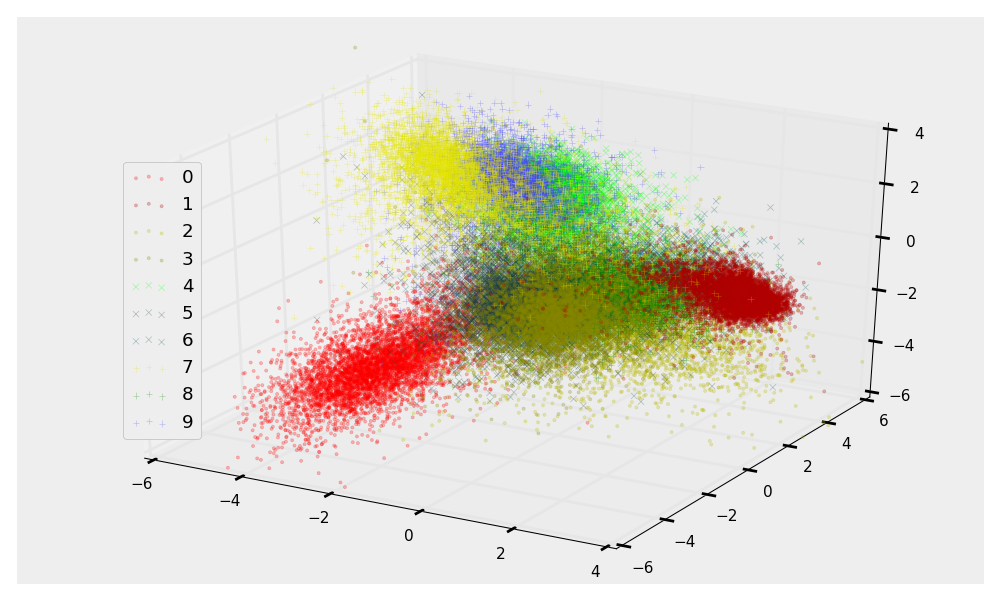
\includegraphics[width=0.9\linewidth]{fig/3d_lda.png}
   \caption{3D LDA 可视化}
\label{fig:3d_lda}
\end{figure*}


表格插入:

\begin{table}[!htbp]
% \resizebox{1.4\linewidth}{!}
  \centering
  \scalebox{1}{
\begin{tabular}{ l || c | c | c | c | c | c | c | c | c | c}
  \hline      
  dim & 2 & 3 & 4 & 5 & 6 & 7 & 8 & 9 & 10 & 20  \\ \hline
  Err. \%  & 100 & 100 &100 &100 &100 &100 &100 &100 &100 &100  \\
  \hline  
\end{tabular}
}
\caption{错误}
\label{tb:lda_knn}
\end{table}

引用 \cite{bishop2006pattern}, 链接: \url{http://fudan.edu.cn}

\bibliographystyle{plain}
\bibliography{report}


\end{document}